%\VignetteEngine{knitr::knitr}
%\VignetteIndexEntry{mixedMem}
\documentclass{article}\usepackage[]{graphicx}\usepackage[]{color}
%% maxwidth is the original width if it is less than linewidth
%% otherwise use linewidth (to make sure the graphics do not exceed the margin)
\makeatletter
\def\maxwidth{ %
  \ifdim\Gin@nat@width>\linewidth
    \linewidth
  \else
    \Gin@nat@width
  \fi
}
\makeatother

\definecolor{fgcolor}{rgb}{0.345, 0.345, 0.345}
\newcommand{\hlnum}[1]{\textcolor[rgb]{0.686,0.059,0.569}{#1}}%
\newcommand{\hlstr}[1]{\textcolor[rgb]{0.192,0.494,0.8}{#1}}%
\newcommand{\hlcom}[1]{\textcolor[rgb]{0.678,0.584,0.686}{\textit{#1}}}%
\newcommand{\hlopt}[1]{\textcolor[rgb]{0,0,0}{#1}}%
\newcommand{\hlstd}[1]{\textcolor[rgb]{0.345,0.345,0.345}{#1}}%
\newcommand{\hlkwa}[1]{\textcolor[rgb]{0.161,0.373,0.58}{\textbf{#1}}}%
\newcommand{\hlkwb}[1]{\textcolor[rgb]{0.69,0.353,0.396}{#1}}%
\newcommand{\hlkwc}[1]{\textcolor[rgb]{0.333,0.667,0.333}{#1}}%
\newcommand{\hlkwd}[1]{\textcolor[rgb]{0.737,0.353,0.396}{\textbf{#1}}}%

\usepackage{framed}
\makeatletter
\newenvironment{kframe}{%
 \def\at@end@of@kframe{}%
 \ifinner\ifhmode%
  \def\at@end@of@kframe{\end{minipage}}%
  \begin{minipage}{\columnwidth}%
 \fi\fi%
 \def\FrameCommand##1{\hskip\@totalleftmargin \hskip-\fboxsep
 \colorbox{shadecolor}{##1}\hskip-\fboxsep
     % There is no \\@totalrightmargin, so:
     \hskip-\linewidth \hskip-\@totalleftmargin \hskip\columnwidth}%
 \MakeFramed {\advance\hsize-\width
   \@totalleftmargin\z@ \linewidth\hsize
   \@setminipage}}%
 {\par\unskip\endMakeFramed%
 \at@end@of@kframe}
\makeatother

\definecolor{shadecolor}{rgb}{.97, .97, .97}
\definecolor{messagecolor}{rgb}{0, 0, 0}
\definecolor{warningcolor}{rgb}{1, 0, 1}
\definecolor{errorcolor}{rgb}{1, 0, 0}
\newenvironment{knitrout}{}{} % an empty environment to be redefined in TeX

\usepackage{alltt}

\linespread{1.6}
\usepackage{amsmath,amsthm,amssymb}
\usepackage[margin= 1in]{geometry} 
\usepackage{natbib, underscore}
\newcommand{\E}{\mathbb{E}}
\usepackage{setspace} 
\renewenvironment{knitrout}{\begin{singlespace}}{\end{singlespace}}
\IfFileExists{upquote.sty}{\usepackage{upquote}}{}
\begin{document}
\title{Fitting Mixed Membership Models using \texttt{mixedMem}}
\author{Y. Samuel Wang and Elena A. Erosheva}
\maketitle

\small
\begin{abstract}
This vignette is a tutorial for the \texttt{mixedMem} R package. \texttt{mixedMem} provides tools for fitting and interpreting mixed membership models. Currently, the package supports multivariate models with binary, multinomial, or rank data (Plackett-Luce distributed). Within a model, each variable can be a different type of distribution and replicates are also supported. This tutorial provides an outline of functions available in the package and a ste-by-step guide for fitting mixed membership models. As an example, we analyze political survey data from the 1983 American National Election Survey Pilot and identify latent ideology blocs within the population.  
\end{abstract}

\normalsize
\section{Mixed Membership Modeling}
\subsection{Mixed Membership Background}
Mixed membership models provide a useful framework for analyzing multivariate data from heterogenous populations \citep{Airoldi2014Handbook}. Similar to mixture models, mixed membership models assume that the overall population is comprised of several latent sub-populations or groups. Mixture models, however, assume that each individual within the population belongs to a single group, whereas mixed membership models allow for an individual to belong to multiple groups simultaneously and explicitly specify an individual's degree of membership in each group. (ELENA TO FILL IN)

Mixed membership models are used to analyze to a wide variety of data types and provide insight into various different scientific problems. Mixed membership analysis of text data \citep{LDA, erosheva2004mixed} can classify documents by topic/subject; analysis of genotype sequences \citep{pritchard2000inference} can estimate genotype frequencies across various origin populations; analysis of survey data \citep{erosheva2007describing, grossManriqueVallier} can cluster survey respondents into interpretable clusters; and analysis of ranked votes \citep{gormley2009grade} can provide insight into latent voting blocs and voting tendencies. The \texttt{mixedMem} package allows for fitting these specific cases of mixed membership models as well as their extensions using a general framework described by \cite{erosheva2004mixed}. The package relies on a variational EM algorithim which will be further described in section \ref{VA}.

\subsection{Illustration and Notation}
For a hypothetical example, consider a survey with J = 3 questions in which 100 high school students (1) rank their favorite classes (rank data), (2) select their favorite TV channel (multinomial data) and (3) indicate whether or not they are on the honor roll (Bernoulli data). Students within the same extracurricular activities/clubs might give similar responses, so in a mixed membership analysis, the latent sub-populations map to the extracurricular groupings. For concreteness, assume the following K = 4 sub-populations fully describe the student's extracurricular activities: athletics, math/science, fine arts and student government. Athletes might be more likely to rank ``Anatomy" and ``Health" among their favorite classes, while students involved in student government might be more likely to rank ``Civics" or ``History" highly.  As is often the case, students may be involved with multiple clubs/activities to varying degrees. If a student is involved in student government and athletics, they might rank their favorite classes as (1. ``Anatomy", 2. ``History" and 3. ``Health"). Thus, using a mixture model framework to classify the student solely as an athlete would fail to represent her full profile. We use $\lambda_i$ to denote the distribution of membership for individual i. $\lambda_i$ is a vector of K elements which are all positive and sum to 1. The membership vector $\lambda$ for the student above might be $\left(\text{athletics} = 0.7, \text{math/science} = 0.0, \text{fine arts} = 0.0, \text{student government} = 0.3\right)$.

For notation, we index each of the students by $i = 1,2, \ldots$ T; in this case T = 100. Variables are indexed by $j = 1,2,\ldots J$ and for each variable we index the number of replicates by $r = 1,2,\ldots R_j$. Since there are only 3 questions in the survey, J, the total number of variables, is 3 and with only 1 replicate each variable $R_j = 1$ for $j = 1,2,3$. For each individual i, variable j and repetition r, we denote the observed response by $X_{i,j,r}$. To accomodate rank data, each individual observation may also consist of multiple ranking levels which we index by $n = 1, \ldots N_{i,j,r}$ (for multinomial and binary data $N_{i,j,r}$ is always 1). For example, the observed ranking of favorite classes (variable 1) for student 10 would be $X_{i = 10, j = 1, r = 1} = \left(\text{``Anatomy", ``History", ``Health"}\right)$. In this case, $N_{i = 10, j = 1, r = 1} = 3$, and $X_{i = 10,j = 1,r = 1,n = 3} =$ ``Civics".    

\subsection{Generative Process}\label{generative}
More formally, for K sub-populations, we assume a mixed membership generating process as follows:

\noindent
For each individual $i = 1,\ldots T$: Draw $\lambda_i$ from a Dirichlet($\alpha$). $\lambda_i$ is a vector of length K which indicates the degree of membership for individual i.
  \begin{itemize}
  \item For each variable $j = 1, \ldots, J$, each replicate $r = 1, \dots, R_j$ and each ranking level $n = 1\ldots, N_{i,j,r}$: Draw $Z_{i,j,r,n}$ from a multinomial(1, $\lambda_i$). $Z_{i,j,r,n}$ determines the sub-population which governs the response for observation $X_{i,j,r,n}$. This is sometimes referred to as the context vector because it determines the context from whicht the individual responds.
  \item For each variable $j = 1, \ldots, J$, each replicate $r = 1, \dots, R_j$ and each ranking level $n = 1\ldots, N_{i,j,r}$: Draw $X_{i,j,r,n}$ from the distribution parameterized by $\theta_{j,Z_{i,j,r,n}}$. Here, $\theta$ is the set of parameters which govern the observations for each sub-population. If variable j is a multinomial or rank distribution with $V_j$ categories/candidates, $\theta_{j,k}$ is a vector of length $V_j$ which parameterizes the responses to variable j for sub-population k. If variable j is a Bernoulli random variable, then $\theta_{j,k}$ is a value which determines the probability of success. 
  \end{itemize}

\section{Variational Inference and the \texttt{mixedMem} Package}\label{VA}

\subsection{Fitting Mixed Membership Models}
When using a mixed membership model, the interest is typically in estimating the sub-population parameters $\theta$, the Dirichlet hyper-parameter $\alpha$ and the latent memberships of individuals $\lambda$. Estimation of these quantities through maximum likelihood or direct posterior inference is computationally intractable in a mixed membership model, so Markov Chain Monte Carlo or variational inference techniques are used instead \citep{airoldi2009mixed}. Most MCMC analyses typically require large amounts of human effort to tune and check the samplers for convergence. Furthermore, in mixed membership models, we must sample a latent membership for each individual and a context vector for each observed response; thus, a mixed membership MCMC analysis becomes very computationally expensive as the number of individuals grows. \texttt{mixedMem} circumvents these difficulties by employing a variational inference which is a computationally attractive, deterministic approach for fitting mixed membership models. Using variational inference allows us to fit larger models and avoids tedious human effort by approximating the true posterior and replacing the MCMC sampling procedure with an optimization problem \citep{beal2003variational}.  

\subsection{Variational Inference}\label{VI}
Instead of working with the intractable true posterior, variational inference uses a more computationally tractable approximate variational distribution. This variational distribution, denoted by Q, is parameterized by $\phi$ and $\delta$ as follows: 

\begin{equation} \label{eq:varDist}
p(\lambda, Z|X) \approx Q(\lambda,Z|\phi, \delta) = \prod_i^T \text{Dirirchlet}(\lambda_i|\phi_i)\prod_j^J \prod_r^{R_j} \prod_n^{N_{i,j,r}}\text{multinomial}(Z_{i,j,r,n}|\delta_{i,j,r,n}).
\end{equation}

The parameters $\phi$ and $\delta$ can be selected to minimize the Kullback-Leibler divergence between the true posterior distribution and the variational distirbution Q \citep{beal2003variational}. This provides an approximate distribution which can be used to carry out posterior inference on the latent variables and posterior means which can be used as point estimates for $\lambda$.

This variational distribution can also be used in an alternative psuedo-likelihood framework, to select the global parameters $\theta$ and $\alpha$. Using Jensen's inequality, the variational distribution can be used to derive a function of $\phi$, $\delta$, $\alpha$ and $\theta$ which is a lower bound on the log-likelihood of our observations:

\begin{equation}\label{eq:Jensen}
p(X|\alpha, \theta) \geq \E_Q\left\{\log\left[p(X,Z, \Lambda)\right]\right\} - \E_Q\left[\log\left[Q(Z, \Lambda|\phi, \delta)\right]\right\}.
\end{equation}

The lower bound on the RHS of equation (\ref{eq:Jensen}) is often called the ELBO for \textbf{E}vidence \textbf{L}ower \textbf{Bo}und. Calculating the LHS of equation (\ref{eq:Jensen}) is intractable, but for a fixed $\phi$ and $\delta$, selecting $\alpha$ and $\theta$ to maximize the lower bound is a tractable alternative to maximum likelihood estimation. 

It can be shown that minimizing the KL Divergence between Q and the true posterior is actually equivalent to maximizing the lower bound in equation (\ref{eq:Jensen}) with respect to $\phi$ and $\delta$ \citep{beal2003variational}. Thus, both tasks of finding an approximate posterior distribution with respect to $\phi$ and $\delta$ and picking psuedo-MLE's $\theta$ and $\alpha$ can be jointly achieved by maximizing the lower bound in equation (\ref{eq:Jensen}). In practice, we maximize this lower bound through a variational EM procedure. In the E-step, we fix $\theta$ and $\alpha$ and minimize the KL divergence between Q and the true posterior with respect to $\phi$ and $\delta$  (this is also equivalent to maximizing the lower bound in equation \ref{eq:Jensen}) through iterative closed form updates. In the M-step, we fix $\phi$ and $\delta$ and select the $\theta$ and $\alpha$ which maximize the lower bound through gradient based methods. The entire procedure iterates between the E-step and the M-step until reaching a local mode. A detailed exposition of variational inference is provided by \cite{jaakkola200110}.

\subsubsection{Label Switching in Mixed Membership Models}
Mixed membership models are only identifiable up to permutatons of the sub-population labels (ie simultaneously permuting the labels for all group memberships and distribution parameters). In an MCMC analysis of mixed membership models, this can be especially pernicious if label switching is present within a sampler \citep{stephens2000dealing}. Because variational inference is a deterministic approach, the final permutation of the labels is only dependent on the initiailization points and does not require special attention during the fitting procedure. However, in order to accurately assess how well a model fits, matching group labels can be a concern when comparing a fitted model to some ground truth or another fitted model. As discussed in section \ref{postProcess}, \texttt{mixedMem} provides functions for dealing with the label permutations to facilitate post-processing.   

\subsubsection{Variational Inference Caveats}
The computational benefits of variational inference, however, do not come for free. The lower bound in equation (\ref{eq:Jensen}), is generally not a strictly convex function, so only convergence to a local mode, not the global mode, is guaranteed. If prior knowledge exists about a specific problem, initializing $\theta$ and $\alpha$ near plausible values is helpful in ensuring that the EM algorithim reaches a reasonable mode. In general though, starting from multiple initialization points and selecting the mode with the largest ELBO is highly recommended. This is also an area where the post-processing tools discussed in section \ref{postProcess} can be useful for determining if candidate modes are conceptually different.

Variational inference also lacks any guarantees on the quality of our approximation. \cite{erosheva2007describing} show that a mixed membership analysis of survey data using a MCMC and variational approach agree well, and, in practice, we see that variational inference provides reasonable and interpretable results in mixed membership models \citep{LDA, erosheva2004mixed, airoldi2009mixed}. However, there are no theoretical guarantees on how good or bad our approximation ultimately is.

\section{Example: Fitting Political Survey Data with \texttt{mixedMem}}
For demonstration, we present a \texttt{mixedMem} analysis of political opinion survey data previously analyzed by  \cite{grossManriqueVallier} as well as \cite{feldman1988structure}. Within this context, identified latent sub-populations might map to ideological blocs. Since individuals often hold to political ideologies to varying degrees, a mixed membership model is particularly appropriate. We utilize same mixed membership model as specified by Gross and Manrique-Vallier and discussed more generally in section \ref{generative}. The model assumes 3 latent sub-populations (K = 3), where individual memberships $\lambda$ are drawn from a dirichlet distribution, the context sub-population Z is drawn from a multinomial(1,$\lambda$) and individual observations are drawn from multinomials governed by the parameters of the respective context sub-population. Gross and Manrique-Vallier specify a fully Bayesian approach, placing prior distributions on both $\theta$ and $\alpha$ and utilize MCMC to estimate the model. This allows for posterior inference on both the latent memberships as well as on $\theta$ and $\alpha$. Our analysis using \texttt{mixedMem} will fit the model using the variational EM algorithim  which allows for posterior inference on $\lambda$ and Z, but only yields point estimates for $\alpha$ and $\theta$. Nonetheless, we will show that the two methods yield comparable results and very similar interpretations.

In the 1983 American National Election Survey Pilot \citep{ANES}, each individual was prompted with various opinion-based statements and was asked to report their agreement with the statement using the categories: ``strongly agree", ``agree but not strongly", ``can't decide", ``disagree but not strongly", and ``strongly disagree". For example, one statement was ``Any person who is willing to work hard has a good chance of succeeding". We specifically study 19 of the statements which were selected by \cite{feldman1988structure} and reanalyzed by \citep{grossManriqueVallier}.  The 19 statements can be grouped into 3 overarching themes: Equality (abbreviated ``EQ" in the data set variable names), Economic Individualism (abbreviated ``IND") and Free Enterprise (abbreviated ``ENT") \citep{feldman1988structure}.  Following the original analysis of \cite{grossManriqueVallier}, we include the 279 complete responses, and combine categories ``agree" with ``strongly agree" and ``disagree"  with ``strongly disagree", leaving the 3 possible responses ``agree" = 0, ``can't decide" = 1, and ``disagree" = 2 to avoid overparameterization. The data is included in \texttt{mixedMem} as \texttt{ANES}; the full text statement for each variable can be accessed through \texttt{help(ANES)}. 

A brief exploratory analysis, shows that of the $279 \times 19 = 5301$ total responses, 3295 responses are ``agree" 1907 are ``disagree" and only 99 are ``can't decide".



\begin{knitrout}
\definecolor{shadecolor}{rgb}{0.969, 0.969, 0.969}\color{fgcolor}\begin{kframe}
\begin{alltt}
\hlkwd{library}\hlstd{(mixedMem)}
\end{alltt}


{\ttfamily\noindent\itshape\color{messagecolor}{\#\# Loading required package: gtools}}\begin{alltt}
\hlkwd{data}\hlstd{(ANES)}
\hlcom{# Dimensions of the data set: 279 individuals with 19 responses each}
\hlkwd{dim}\hlstd{(ANES)}
\end{alltt}
\begin{verbatim}
## [1] 279  19
\end{verbatim}
\begin{alltt}
\hlcom{# The 19 variables and their categories}
\hlcom{# The specific statements for each variable can be found using help(ANES)}
\hlcom{# Variables titled EQ are about Equality}
\hlcom{# Variables titled IND are about Econonic Individualism}
\hlcom{# Variables titled ENT are about Free Enterprise}
\hlkwd{colnames}\hlstd{(ANES)}
\end{alltt}
\begin{verbatim}
##  [1] "EQ1"  "EQ2"  "EQ3"  "EQ4"  "EQ5"  "EQ6"  "EQ7"  "IND1" "IND2" "IND3"
## [11] "IND4" "IND5" "IND6" "ENT1" "ENT2" "ENT3" "ENT4" "ENT5" "ENT6"
\end{verbatim}
\begin{alltt}
\hlcom{# Distribution of responses}
\hlkwd{table}\hlstd{(}\hlkwd{unlist}\hlstd{(ANES))}
\end{alltt}
\begin{verbatim}
## 
##    0    1    2 
## 3295   99 1907
\end{verbatim}
\end{kframe}
\end{knitrout}

\subsection*{Step 1: Initializing the \texttt{mixedMemModel} Object}
To fit a mixed membership model, we must first initialize a \texttt{mixedMemModel} object using the class constructor. The \texttt{mixedMemModel} object contains the dimensions of our mixed membership model, the observed data and initialization points for $\alpha$ and $\theta$. Creating a \texttt{mixedMemModel} object provides a vehicle for passing this information to the \texttt{mmVarFit} function in step 2 similar to how one might specify the formula for an \texttt{lm} object. Although initialization points for $\phi$ and $\delta$ can be passed to the constructor as well, these by default are initialized uniformly across the sub-populations. Unless there is very strong prior knowledge, we recommend that the default values be used. For this particular model, all the variables are multinomials; an example showing an initialization of mixed data types can be accessed through \texttt{help(mixedMemModel)}.

As mentioned previously, because the lower bound function is not convex, different initializations may result in convergence to different local modes. After initializing at various point, we found that the initialization of $\alpha = \left(.2, .2, .2\right)$ and $\theta \sim \text{Dirichlet}(.8)$ using seed 123 resulted in the highest lower bound at convergnce.  

\begin{knitrout}
\definecolor{shadecolor}{rgb}{0.969, 0.969, 0.969}\color{fgcolor}\begin{kframe}
\begin{alltt}
\hlcom{# Sample Size}
\hlstd{Total} \hlkwb{<-} \hlnum{279}
\hlcom{# Number of variables}
\hlstd{J} \hlkwb{<-} \hlnum{19}
\hlcom{# we only have one replicate for each of the variables}
\hlstd{Rj} \hlkwb{<-} \hlkwd{rep}\hlstd{(}\hlnum{1}\hlstd{, J)}
\hlcom{# Nijr indicates the number of ranking levels for each variable.}
\hlcom{# Since all our data is multinomial it should be an array of all 1s}
\hlstd{Nijr} \hlkwb{<-} \hlkwd{array}\hlstd{(}\hlnum{1}\hlstd{,} \hlkwc{dim} \hlstd{=} \hlkwd{c}\hlstd{(Total, J,} \hlkwd{max}\hlstd{(Rj)))}
\hlcom{# Number of sub-populations}
\hlstd{K} \hlkwb{<-} \hlnum{3}
\hlcom{# There are 3 choices for each of the variables ranging from 0 to 2.}
\hlstd{Vj} \hlkwb{<-} \hlkwd{rep}\hlstd{(}\hlnum{3}\hlstd{, J)}
\hlcom{# we initialize alpha to .2}
\hlstd{alpha} \hlkwb{<-} \hlkwd{rep}\hlstd{(}\hlnum{.2}\hlstd{, K)}
\hlcom{# All variables are multinomial}
\hlstd{dist} \hlkwb{<-} \hlkwd{rep}\hlstd{(}\hlstr{"multinomial"}\hlstd{, J)}
\hlcom{# obs are the observed responses. it is a 4-d array indexed by i,j,r,n}
\hlcom{# note that obs ranges from 0 to 2 for each response}
\hlstd{obs} \hlkwb{<-} \hlkwd{array}\hlstd{(}\hlnum{0}\hlstd{,} \hlkwc{dim} \hlstd{=} \hlkwd{c}\hlstd{(Total, J,} \hlkwd{max}\hlstd{(Rj),} \hlkwd{max}\hlstd{(Nijr)))}
\hlstd{obs[,,}\hlnum{1}\hlstd{,}\hlnum{1}\hlstd{]} \hlkwb{<-} \hlkwd{as.matrix}\hlstd{(ANES)}

\hlcom{# Initialize theta randomly with Dirichlet distributions}
\hlkwd{set.seed}\hlstd{(}\hlnum{123}\hlstd{)}
\hlstd{theta} \hlkwb{<-} \hlkwd{array}\hlstd{(}\hlnum{0}\hlstd{,} \hlkwc{dim}\hlstd{=} \hlkwd{c}\hlstd{(J,K,}\hlkwd{max}\hlstd{(Vj)))}
\hlkwa{for}\hlstd{(j} \hlkwa{in} \hlnum{1}\hlopt{:}\hlstd{J)}
\hlstd{\{}
    \hlstd{theta[j,,]} \hlkwb{<-} \hlkwd{rdirichlet}\hlstd{(K,}\hlkwd{rep}\hlstd{(}\hlnum{.8}\hlstd{,Vj[j]))}
\hlstd{\}}

\hlcom{# Create the mixedMemModel}
\hlcom{# This object encodes the initialization points for the variational EM algorithim}
\hlcom{# and also encodes the observed parameters and responses}
\hlstd{initial} \hlkwb{<-} \hlkwd{mixedMemModel}\hlstd{(}\hlkwc{Total} \hlstd{= Total,} \hlkwc{J} \hlstd{= J,} \hlkwc{Rj} \hlstd{= Rj,}
                         \hlkwc{Nijr} \hlstd{= Nijr,} \hlkwc{K} \hlstd{= K,} \hlkwc{Vj} \hlstd{= Vj,} \hlkwc{alpha} \hlstd{= alpha,}
                         \hlkwc{theta} \hlstd{= theta,} \hlkwc{dist} \hlstd{= dist,} \hlkwc{obs} \hlstd{= obs)}
\end{alltt}
\end{kframe}
\end{knitrout}

\subsection*{Step 2: Fitting the Model}
Now we can fit the model using the \texttt{mmVarFit} function. When we call \texttt{mmVarFit}, the function first checks for internal consistency in the input model, \texttt{initial} (ie. it checks whether the dimensions of the observation match the specified number of variables, etc). If the model check passes, the function begins to iterate through the E-step and M-step described in Subsection \ref{VI}. When the algorithim converges, \texttt{mmVarFit} prints the value of the lower bound at convergence as well as the number of EM iterations needed for convergence.

\begin{knitrout}
\definecolor{shadecolor}{rgb}{0.969, 0.969, 0.969}\color{fgcolor}\begin{kframe}
\begin{alltt}
\hlkwd{computeELBO}\hlstd{(initial)}
\end{alltt}
\begin{verbatim}
## [1] -16810.18
\end{verbatim}
\begin{alltt}
\hlstd{st} \hlkwb{=} \hlkwd{proc.time}\hlstd{()}
\hlstd{out} \hlkwb{<-} \hlkwd{mmVarFit}\hlstd{(initial)}
\end{alltt}
\begin{verbatim}
## [1] "Model Check: Ok!"
## [1] "<== Beginning Variational Inference ==>"
## Fit Complete! Elbo: -3122.89 Iter: 103
\end{verbatim}
\begin{alltt}
\hlstd{end} \hlkwb{=} \hlkwd{proc.time}\hlstd{()}
\hlkwd{computeELBO}\hlstd{(out)}
\end{alltt}
\begin{verbatim}
## [1] -3122.886
\end{verbatim}
\begin{alltt}
\hlstd{time} \hlkwb{=} \hlstd{end} \hlopt{-} \hlstd{st}
\end{alltt}
\end{kframe}
\end{knitrout}

Notice that the lower bound (our objective function) is \ensuremath{-1.681018\times 10^{4}} at the initialized points and is \ensuremath{-3122.89} at convergence. On a laptop (quad-core 2.4 GHZ with 12 GB of RAM), fitting the entire model took only 10.61 seconds, significantly faster than a full MCMC analysis.  
We can also view a quick summary of the fit model using the \texttt{summary} function.

\begin{knitrout}
\definecolor{shadecolor}{rgb}{0.969, 0.969, 0.969}\color{fgcolor}\begin{kframe}
\begin{alltt}
\hlkwd{summary}\hlstd{(out)}
\end{alltt}
\begin{verbatim}
## ==Summary for Mixed Membership Model==
## Total: 279		 K: 3		 ELBO: -3122.89
## 
##  Variable   Variable Type     Replicates     Categories  
##    1        multinomial       1              3           
##    2        multinomial       1              3           
##    3        multinomial       1              3           
##    4        multinomial       1              3           
##    5        multinomial       1              3           
##    6        multinomial       1              3           
##    7        multinomial       1              3           
##    8        multinomial       1              3           
##    9        multinomial       1              3           
##    10       multinomial       1              3           
##    11       multinomial       1              3           
##    12       multinomial       1              3           
##    13       multinomial       1              3           
##    14       multinomial       1              3           
##    15       multinomial       1              3           
##    16       multinomial       1              3           
##    17       multinomial       1              3           
##    18       multinomial       1              3           
##    19       multinomial       1              3
\end{verbatim}
\end{kframe}
\end{knitrout}

\subsection*{Step 3: Post-Processing}\ref{PostProcess}
In many cases, we may be interested in comparing our fitted model to some ground truth or comparing various runs with different starting values. Since the model is invariant to label permutations, we use the \texttt{findLabels} function to match our sub-population labels to the ground truth to facilitate comparison. In this case, we are interested in comparing our fitted values with the posterior means from the original MCMC analysis of \cite{grossManriqueVallier}. The \texttt{findLabels} function finds the permutation of labels which minimizes the weighted squared error shown in equation (\ref{eq:loss}). Once we have found the optimal permutation, we then permute the sub-population labels using the \texttt{permuteLabels} function. 

\begin{equation}\label{eq:loss}
Loss = \sum_i^{T} \sum_j^J \frac{\hat \alpha_k}{\hat \alpha_0} \sum_v^{V_j}(\hat \theta_{j,k,v} - \theta_{j,k,v})^2
\end{equation}

Where $\hat \alpha_0 = \sum_k \alpha_k$.

\begin{knitrout}
\definecolor{shadecolor}{rgb}{0.969, 0.969, 0.969}\color{fgcolor}\begin{kframe}
\begin{alltt}
\hlcom{#read in GM estimates}
\hlkwd{data}\hlstd{(gmv_theta)}
\hlcom{#}
\hlstd{optimal.perm} \hlkwb{<-} \hlkwd{findLabels}\hlstd{(out, gmv_theta)}
\hlcom{# display the permutation as well as the weighted squared error loss}
\hlstd{optimal.perm}
\end{alltt}
\begin{verbatim}
## $perm
## [1] 3 2 1
## 
## $loss
## [1] 5.205028
\end{verbatim}
\begin{alltt}
\hlcom{# save object with permuted labels}
\hlstd{out.permute} \hlkwb{<-} \hlkwd{permuteLabels}\hlstd{(out, optimal.perm}\hlopt{$}\hlstd{perm)}
\end{alltt}
\end{kframe}
\end{knitrout}

\subsection{Step 4: Interpretation}
Visualizations of the fitted model can be highly context specific, but we show a few visualizations and tools which may be of general interest below.
\subsubsection{Visual Representation of $\hat \theta$}
We can now plot our estimated $\hat \theta$ values and compare them to the values found in the original analysis. In the plots shown below, each row of plots represents an individual question, the columns represent each of the identified sub-populations and the plots show the sub-populations's response probability for each variable. The black bars indicate the values estimated using \texttt{mixedMem} and the green dots indicate the values reported by \citep{grossManriqueVallier}. Note that Gross and Manrique-Vallier do not report values for group 3 for reasons discussed later in this section. Recall that 0 indicates ``agree" and 2 indicates ``disagree".

\begin{knitrout}
\definecolor{shadecolor}{rgb}{0.969, 0.969, 0.969}\color{fgcolor}\begin{kframe}
\begin{alltt}
\hlkwd{vizTheta}\hlstd{(out.permute, gmv_theta,} \hlkwc{varNames} \hlstd{=} \hlkwd{colnames}\hlstd{(ANES),}
         \hlkwc{groupNames} \hlstd{=} \hlkwd{c}\hlstd{(}\hlstr{"Conservative"}\hlstd{,} \hlstr{"Liberal"}\hlstd{,} \hlstr{"Undecided"}\hlstd{))}
\end{alltt}
\end{kframe}\begin{figure}

{\centering 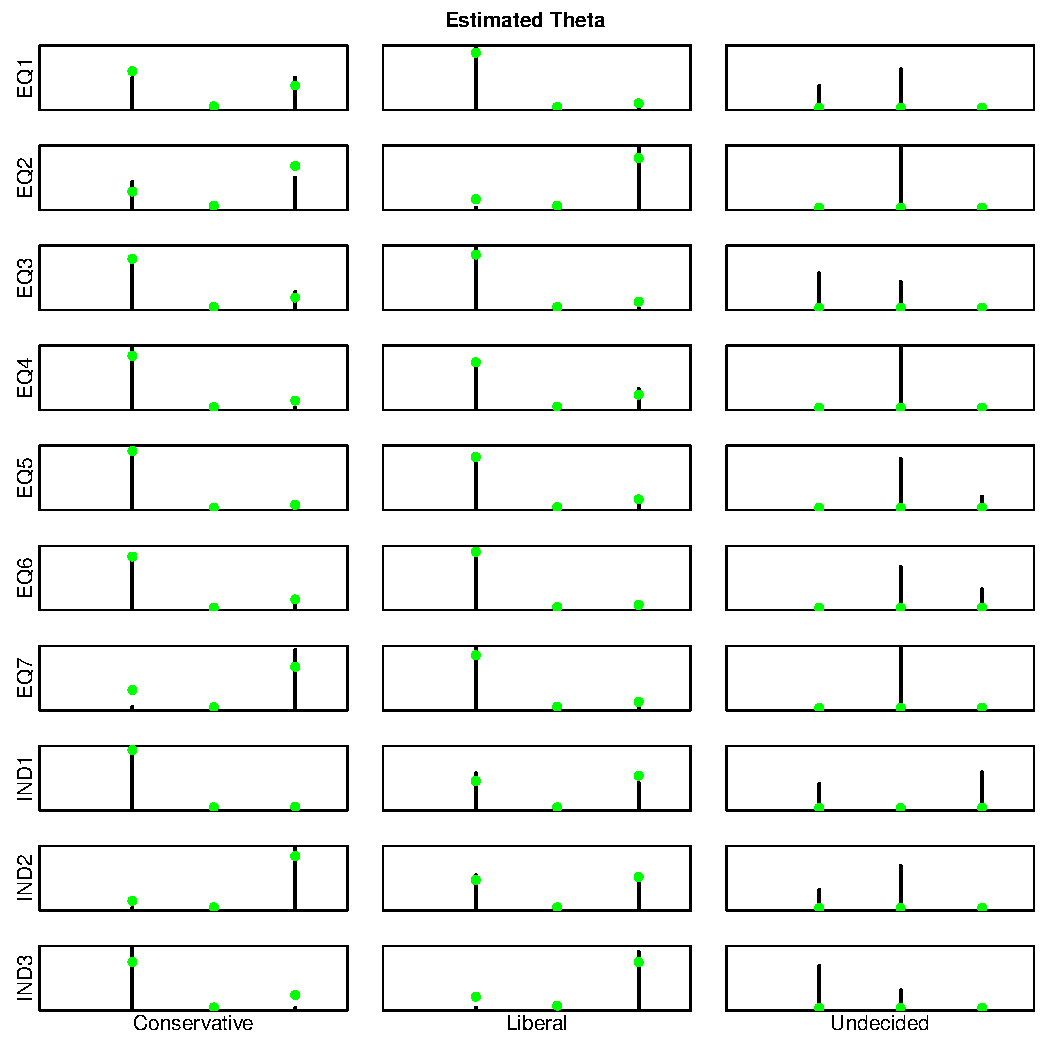
\includegraphics[width=\maxwidth]{figure/thetaPlot-1} 

}

\caption[Variational Estimates shown in black, GMV estimates shown in green]{Variational Estimates shown in black, GMV estimates shown in green\label{fig:thetaPlot1}}
\end{figure}

\begin{figure}

{\centering 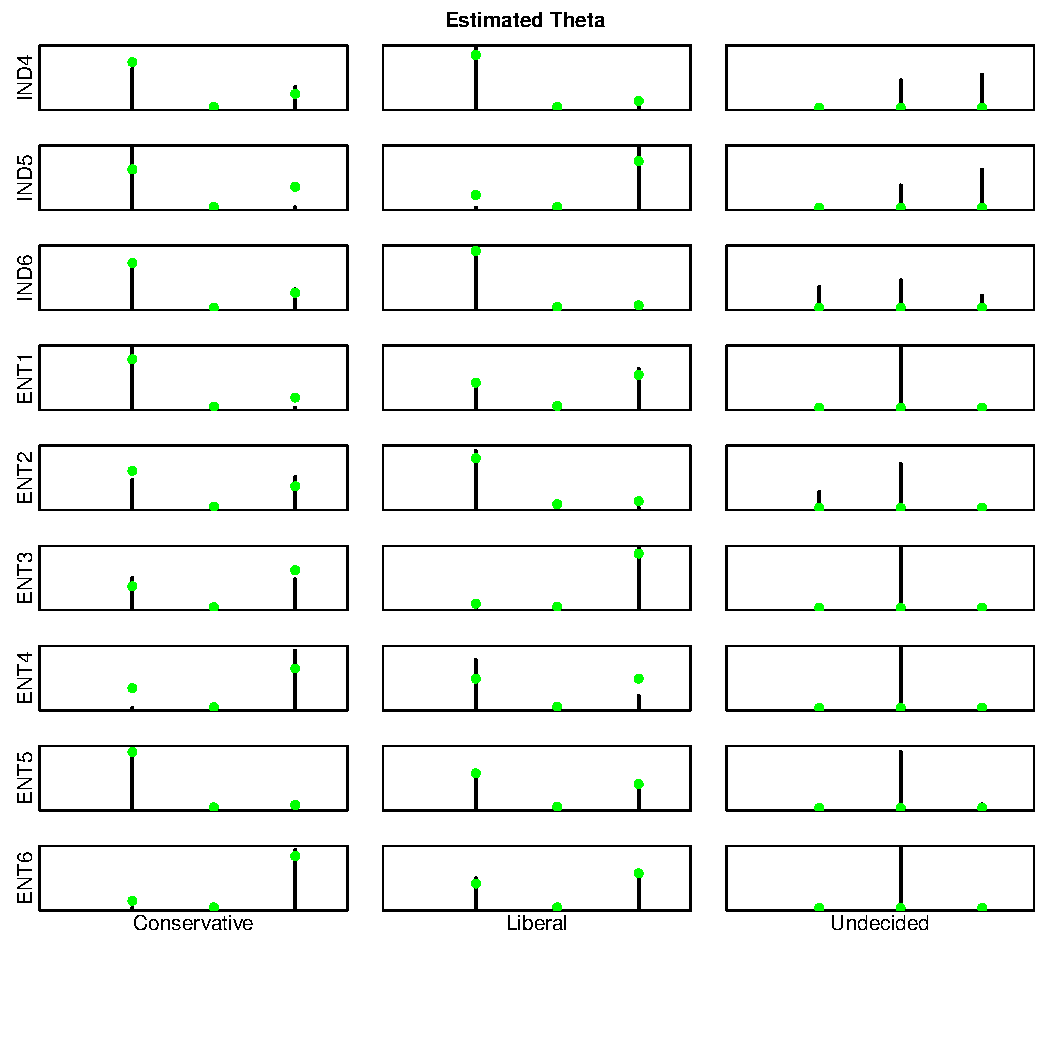
\includegraphics[width=\maxwidth]{figure/thetaPlot-2} 

}

\caption[Variational Estimates shown in black, GMV estimates shown in green]{Variational Estimates shown in black, GMV estimates shown in green\label{fig:thetaPlot2}}
\end{figure}


\end{knitrout}

When examining the estimates of $\hat \theta$, we can see that of all 19 variables, the statements most likely to elicit agreement from sub-population 1 are statement \texttt{IND1} (``Any person who is willing to work hard has a good chance of succeeding"), \texttt{IND3} (``Most people who don't get ahead should not blame the system; they really have only themselves to blame") and \texttt{ENT1} (``The less government gets involved with business and the economy, the better off this country will be"). Using traditional political ideology labels, sub-population 1 could be identified as the conservative bloc. In figure \ref{fig:consProp}, columns shown in green indicate question to which sub-population 1 is more likely to agree ($\theta_{j,1,1} \geq .5$) and columns shown in red indicate questions to which the sub-population is not likely to agree.

\begin{knitrout}
\definecolor{shadecolor}{rgb}{0.969, 0.969, 0.969}\color{fgcolor}\begin{kframe}
\begin{alltt}
\hlstd{pop1VarOrder} \hlkwb{=} \hlkwd{colnames}\hlstd{(ANES)[}\hlkwd{order}\hlstd{(out.permute}\hlopt{$}\hlstd{theta[,}\hlnum{1}\hlstd{,}\hlnum{1}\hlstd{],} \hlkwc{decreasing} \hlstd{= T)]}
\hlstd{pop1VarAgree} \hlkwb{=} \hlkwd{sort}\hlstd{(out.permute}\hlopt{$}\hlstd{theta[,}\hlnum{1}\hlstd{,}\hlnum{1}\hlstd{],} \hlkwc{decreasing} \hlstd{= T)}
\hlkwd{barplot}\hlstd{(}\hlkwc{height} \hlstd{= pop1VarAgree,} \hlkwc{names.arg} \hlstd{= pop1VarOrder,}
        \hlkwc{main} \hlstd{=} \hlstr{"Propensity to Agree"}\hlstd{,}
        \hlkwc{cex.names} \hlstd{=} \hlnum{.7}\hlstd{,} \hlkwc{las} \hlstd{=} \hlnum{2}\hlstd{,} \hlkwc{sub} \hlstd{=} \hlstr{"Conservative Bloc"}\hlstd{,}
        \hlkwc{ylab} \hlstd{=} \hlkwd{expression}\hlstd{(}\hlkwd{paste}\hlstd{(theta[}\hlstr{"j,1,1"}\hlstd{])),}
        \hlkwc{col} \hlstd{=}\hlkwd{ifelse}\hlstd{(pop1VarAgree} \hlopt{>} \hlnum{.5}\hlstd{,} \hlstr{"forestgreen"}\hlstd{,} \hlstr{"darkred"}\hlstd{))}
\end{alltt}
\end{kframe}\begin{figure}

{\centering 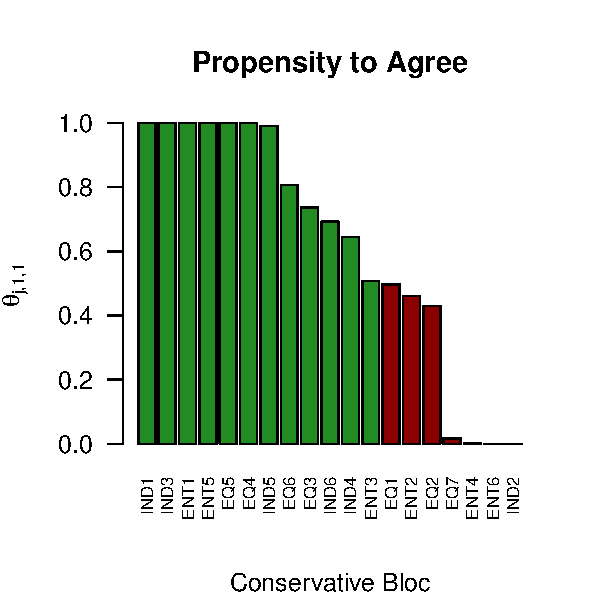
\includegraphics[width=\maxwidth]{figure/consProp-1} 

}

\caption[Propensity to agree with each opinion-based statement for the conservative bloc]{Propensity to agree with each opinion-based statement for the conservative bloc\label{fig:consProp}}
\end{figure}


\end{knitrout}

We can see that for sub-population 2, the statements most likely to elicit agreement are statements \texttt{EQ7} (``One of the big problems in this country is that we don't give everyone an equal chance"), \texttt{IND6} (``Even if people try hard, they often cannot reach their goals
") and \texttt{EQ1} (``If people were treated more equally in this country, we would have many fewer problems
"). Sub-population 2 could be identified as the liberal bloc. 

\begin{knitrout}
\definecolor{shadecolor}{rgb}{0.969, 0.969, 0.969}\color{fgcolor}\begin{kframe}
\begin{alltt}
\hlstd{pop2VarOrder} \hlkwb{=} \hlkwd{colnames}\hlstd{(ANES)[}\hlkwd{order}\hlstd{(out.permute}\hlopt{$}\hlstd{theta[,}\hlnum{2}\hlstd{,}\hlnum{1}\hlstd{],} \hlkwc{decreasing} \hlstd{= T)]}
\hlstd{pop2VarAgree} \hlkwb{=} \hlkwd{sort}\hlstd{(out.permute}\hlopt{$}\hlstd{theta[,}\hlnum{2}\hlstd{,}\hlnum{1}\hlstd{],} \hlkwc{decreasing} \hlstd{= T)}
\hlkwd{barplot}\hlstd{(}\hlkwc{height} \hlstd{= pop2VarAgree,}
        \hlkwc{names.arg} \hlstd{= pop2VarOrder,} \hlkwc{main} \hlstd{=} \hlstr{"Propensity to Agree"}\hlstd{,}
        \hlkwc{cex.names} \hlstd{=} \hlnum{.7}\hlstd{,} \hlkwc{las} \hlstd{=} \hlnum{2}\hlstd{,} \hlkwc{sub} \hlstd{=} \hlstr{"Liberal Bloc"}\hlstd{,}
        \hlkwc{ylab} \hlstd{=} \hlkwd{expression}\hlstd{(}\hlkwd{paste}\hlstd{(theta[}\hlstr{"j,2,1"}\hlstd{])),}
        \hlkwc{col} \hlstd{=}\hlkwd{ifelse}\hlstd{(pop2VarAgree} \hlopt{>} \hlnum{.5}\hlstd{,} \hlstr{"forestgreen"}\hlstd{,} \hlstr{"darkred"}\hlstd{))}
\end{alltt}
\end{kframe}\begin{figure}

{\centering 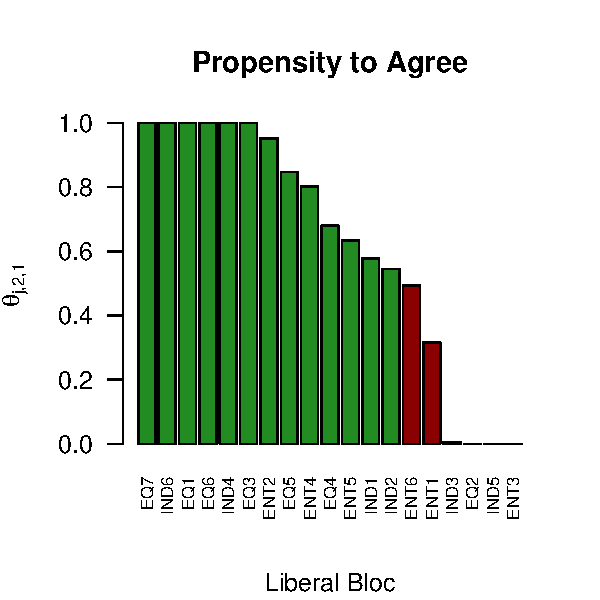
\includegraphics[width=\maxwidth]{figure/unnamed-chunk-7-1} 

}

\caption[Propensity to agree with each opinion-based statement for the liberal bloc]{Propensity to agree with each opinion-based statement for the liberal bloc\label{fig:unnamed-chunk-7}}
\end{figure}


\end{knitrout}

We also observe, that sub-population 3 has a much higher propensity to respond ``can't decide" then sub-populations 1 or 2. The 5 individuals with particularly large membership in group 3 responded ``can't decide" 42 times. This is particularly salient since there are only 99 ``can't decide" responses in the entire sample. Thus, sub-population 3 could be identified as the undecided bloc. 

\begin{knitrout}
\definecolor{shadecolor}{rgb}{0.969, 0.969, 0.969}\color{fgcolor}\begin{kframe}
\begin{alltt}
\hlcom{# Point estimates for lambda}
\hlstd{lambda.point} \hlkwb{<-} \hlstd{out.permute}\hlopt{$}\hlstd{phi}\hlopt{/}\hlkwd{rowSums}\hlstd{(out.permute}\hlopt{$}\hlstd{phi)}
\hlcom{# number of individuals which exhibit more than .3 degree of membership}
\hlcom{# in the undecided group}
\hlkwd{sum}\hlstd{(lambda.point[,}\hlnum{3}\hlstd{]}\hlopt{>=}\hlnum{.3}\hlstd{)}
\end{alltt}
\begin{verbatim}
## [1] 5
\end{verbatim}
\begin{alltt}
\hlcom{# number of can not decide responses from those with high membership in undecided group}
\hlkwd{sum}\hlstd{(ANES[}\hlkwd{which}\hlstd{(lambda.point[,}\hlnum{3}\hlstd{]}\hlopt{>=}\hlnum{.3}\hlstd{),]}\hlopt{==}\hlnum{1}\hlstd{)}
\end{alltt}
\begin{verbatim}
## [1] 42
\end{verbatim}
\end{kframe}
\end{knitrout}

\subsubsection{Interpretation of $\hat \alpha$}
When examining the fitted value of $\hat \alpha$, we see that the conservatives and liberals are the 2 dominant groups with the undecided group comprising a much smaller portion of the population. Also, the large values of $\hat \alpha_1$ and $\hat \alpha_2$, indicate a high level of mixing between those sub-populations which will be further discussed below.  Since the estimated relative frequency of the undecided bloc is less than 1\%, we focus our interpretation of the other two blocs dominant blocs.

\begin{knitrout}
\definecolor{shadecolor}{rgb}{0.969, 0.969, 0.969}\color{fgcolor}\begin{kframe}
\begin{alltt}
\hlstd{relativeFrequency} \hlkwb{=} \hlstd{out.permute}\hlopt{$}\hlstd{alpha}\hlopt{/}\hlkwd{sum}\hlstd{(out.permute}\hlopt{$}\hlstd{alpha)}
\end{alltt}
\end{kframe}
\end{knitrout}

% latex table generated in R 3.1.2 by xtable 1.7-4 package
% Wed Feb 04 21:09:31 2015
\begin{table}[ht]
\centering
\begin{tabular}{rrrr}
  \hline
 & Conservatives & Liberals & Undecided \\ 
  \hline
Estimated Alpha & 3.617 & 3.448 & 0.029 \\ 
  Estimate Relative Frequency & 0.510 & 0.486 & 0.004 \\ 
   \hline
\end{tabular}
\caption{Variational Estimates of Alpha} 
\end{table}


\subsubsection{Using Hellinger Distance to Determine Defining Characteristics for Each Bloc}
We might also be interested in seeing which questions are the most polarizing (the questions to which a conservative is most likely to respond differently than a liberal). These particular value statements provide insight into defining what makes a conservative and what makes a liberal. We use the Hellinger distance, a measure of the difference between distributions, to compare the conservative and liberal response probabilities for each question. Hellinger distance is defined as

\begin{equation}
H(P,Q) = \frac{1}{\sqrt{2}}\sqrt{\sum_i \left(\sqrt{p_i} - \sqrt{q_i}\right)^2}.
\end{equation}

We can see that the three most polarizing questions as measured by the Hellinger distance between the two response probabilities are statements \texttt{IND5} (``If people work hard, they almost always get what they want"), \texttt{IND3} (``Most people who don't get ahead should not blame the system; they really have only themselves to blame") and \texttt{EQ7} (``One of the big problems in this country is that we don't give everyone an equal chance"). Thus, it would seem that the most polarizing issues in 1983 revolved around access and opportunity for advancement.

\begin{knitrout}
\definecolor{shadecolor}{rgb}{0.969, 0.969, 0.969}\color{fgcolor}\begin{kframe}
\begin{alltt}
\hlstd{hellingerDist} \hlkwb{=} \hlstd{(}\hlnum{1}\hlopt{/}\hlkwd{sqrt}\hlstd{(}\hlnum{2}\hlstd{))}\hlopt{*}\hlkwd{sqrt}\hlstd{(}\hlkwd{rowSums}\hlstd{((}\hlkwd{sqrt}\hlstd{(out.permute}\hlopt{$}\hlstd{theta[,}\hlnum{1}\hlstd{,])}
                                          \hlopt{-} \hlkwd{sqrt}\hlstd{(out.permute}\hlopt{$}\hlstd{theta[,}\hlnum{2}\hlstd{,]))}\hlopt{^}\hlnum{2}\hlstd{))}
\hlkwd{barplot}\hlstd{(}\hlkwd{sort}\hlstd{(hellingerDist,} \hlkwc{decreasing} \hlstd{= T),} \hlkwc{names.arg} \hlstd{=} \hlkwd{colnames}\hlstd{(ANES)[}\hlkwd{order}\hlstd{(hellingerDist,} \hlkwc{decreasing} \hlstd{= T)],}
        \hlkwc{main} \hlstd{=} \hlstr{"Hellinger Distance"}\hlstd{,}
        \hlkwc{cex.names} \hlstd{=} \hlnum{.7}\hlstd{,} \hlkwc{las} \hlstd{=} \hlnum{2}\hlstd{,} \hlkwc{ylab} \hlstd{=} \hlstr{"Hellinger Distance"}\hlstd{,}
        \hlkwc{ylim} \hlstd{=} \hlkwd{c}\hlstd{(}\hlnum{0}\hlstd{,}\hlnum{1}\hlstd{))}
\hlkwd{mtext}\hlstd{(}\hlstr{"Between Conservatives and Liberals"}\hlstd{)}
\end{alltt}
\end{kframe}\begin{figure}

{\centering 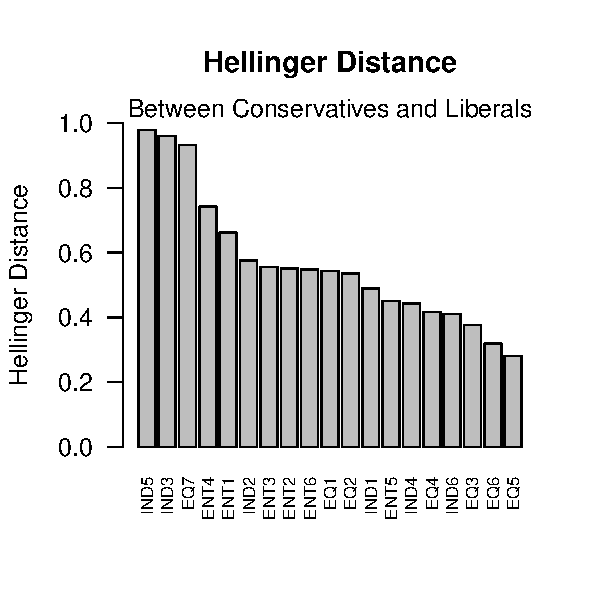
\includegraphics[width=\maxwidth]{figure/unnamed-chunk-11-1} 

}

\caption[Using Hellinger distance indicates that the most polarizing issues involved opportunity for advancement]{Using Hellinger distance indicates that the most polarizing issues involved opportunity for advancement\label{fig:unnamed-chunk-11}}
\end{figure}

\begin{kframe}\begin{alltt}
\hlkwd{colnames}\hlstd{(ANES)[}\hlkwd{order}\hlstd{(hellingerDist,} \hlkwc{decreasing} \hlstd{= T)][}\hlnum{1}\hlopt{:}\hlnum{3}\hlstd{]}
\end{alltt}
\begin{verbatim}
## [1] "IND5" "IND3" "EQ7"
\end{verbatim}
\end{kframe}
\end{knitrout}

\subsection{Visualizing Group Dispersion}



For the groups memberships for individuals, we use the posterior mean, $\frac{\hat \phi_i}{\sum_k \hat \phi_{i,k}}$ as point estimates for $\lambda_i$. Plotting the poster mean of membership in the conservative bloc below, we can see a fair amount of intra-individual mixing. 139 out of the 279 individuals have estimated memberships of at least 40\% in both the conservative and liberal blocs. This is not particularly suprising since we observed relatively large values of $\hat \alpha_1$ and $\hat \alpha_2$.

\begin{knitrout}
\definecolor{shadecolor}{rgb}{0.969, 0.969, 0.969}\color{fgcolor}\begin{kframe}
\begin{alltt}
\hlstd{estimatedLambda} \hlkwb{=} \hlstd{out.permute}\hlopt{$}\hlstd{phi}\hlopt{/}\hlkwd{rowSums}\hlstd{(out.permute}\hlopt{$}\hlstd{phi)}
\hlcom{# number of individuals with at least 40% membership in}
\hlcom{# both conservative and liberal blocs}
\hlkwd{sum}\hlstd{(estimatedLambda[,}\hlnum{1}\hlstd{]}\hlopt{>}\hlnum{.4} \hlopt{&} \hlstd{estimatedLambda[,}\hlnum{2}\hlstd{]} \hlopt{>}\hlnum{.4}\hlstd{)}
\end{alltt}
\begin{verbatim}
## [1] 139
\end{verbatim}
\end{kframe}
\end{knitrout}

We can also plot the ``empirical CDF" of estimated membership in conservative bloc as shown in figure \ref{fig:posteriorMem}. Since the marginal distribution of a Dirichlet distribution is a beta, we can also plot the 95\% credible intervals for the posterior membership in the conservative bloc. We observe that there is still a relatively large amount of uncertainty in the membership of each individual.


\begin{knitrout}
\definecolor{shadecolor}{rgb}{0.969, 0.969, 0.969}\color{fgcolor}\begin{kframe}
\begin{alltt}
\hlstd{index} \hlkwb{=} \hlkwd{order}\hlstd{(estimatedLambda[,}\hlnum{1}\hlstd{])}

\hlcom{# variance of posterior membership in conservative bloc}
\hlstd{var.Mem} \hlkwb{=} \hlstd{out.permute}\hlopt{$}\hlstd{phi[,}\hlnum{1}\hlstd{]}\hlopt{*}\hlstd{(}\hlkwd{rowSums}\hlstd{(out.permute}\hlopt{$}\hlstd{phi)}\hlopt{-}
                                 \hlstd{out.permute}\hlopt{$}\hlstd{phi[,}\hlnum{1}\hlstd{])}\hlopt{/}
  \hlstd{(}\hlkwd{rowSums}\hlstd{(out.permute}\hlopt{$}\hlstd{phi)}\hlopt{^}\hlnum{2}\hlopt{*}\hlstd{(}\hlkwd{rowSums}\hlstd{(out.permute}\hlopt{$}\hlstd{phi)}\hlopt{+}\hlnum{1}\hlstd{))}
\hlcom{# plot posterior means}
\hlkwd{plot}\hlstd{(}\hlkwd{sort}\hlstd{(estimatedLambda[,}\hlnum{1}\hlstd{]),} \hlkwc{pch} \hlstd{=} \hlnum{19}\hlstd{,}
     \hlkwc{main} \hlstd{=} \hlstr{"Posterior Membership in Conservative Bloc"}\hlstd{,}
     \hlkwc{ylab} \hlstd{=} \hlstr{"Posterior Membership"}\hlstd{,} \hlkwc{xlab} \hlstd{=} \hlstr{"Individual"}\hlstd{,}
     \hlkwc{cex} \hlstd{=} \hlnum{.8}\hlstd{,} \hlkwc{ylim} \hlstd{=} \hlkwd{c}\hlstd{(}\hlnum{0}\hlstd{,}\hlnum{1}\hlstd{))}

\hlcom{# marginal distirbution of Dirichlet, is Beta distribution, so we can get posterior CI}
\hlcom{# plot posterior 90% CI}
\hlstd{ci_90} \hlkwb{=} \hlkwd{qbeta}\hlstd{(}\hlnum{.975}\hlstd{, out.permute}\hlopt{$}\hlstd{phi[index,}\hlnum{1}\hlstd{],} \hlkwd{rowSums}\hlstd{(out.permute}\hlopt{$}\hlstd{phi[index,}\hlkwd{c}\hlstd{(}\hlnum{2}\hlopt{:}\hlnum{3}\hlstd{)]))}
\hlstd{ci_10} \hlkwb{=} \hlkwd{qbeta}\hlstd{(}\hlnum{.025}\hlstd{, out.permute}\hlopt{$}\hlstd{phi[index,}\hlnum{1}\hlstd{],} \hlkwd{rowSums}\hlstd{(out.permute}\hlopt{$}\hlstd{phi[index,}\hlkwd{c}\hlstd{(}\hlnum{2}\hlopt{:}\hlnum{3}\hlstd{)]))}
\hlkwd{lines}\hlstd{(ci_90,} \hlkwc{lty} \hlstd{=} \hlnum{2}\hlstd{,} \hlkwc{col} \hlstd{=} \hlstr{"red"}\hlstd{)}
\hlkwd{lines}\hlstd{(ci_10,} \hlkwc{lty} \hlstd{=} \hlnum{2}\hlstd{,} \hlkwc{col} \hlstd{=} \hlstr{"red"}\hlstd{)}
\hlkwd{legend}\hlstd{(}\hlstr{"bottomright"}\hlstd{,} \hlkwc{legend} \hlstd{=} \hlkwd{c}\hlstd{(}\hlstr{"posterior mean"}\hlstd{,} \hlstr{"90% CI"}\hlstd{),} \hlkwc{pch} \hlstd{=} \hlkwd{c}\hlstd{(}\hlnum{19}\hlstd{,} \hlnum{NA}\hlstd{),}
       \hlkwc{lty} \hlstd{=} \hlkwd{c}\hlstd{(}\hlnum{NA}\hlstd{,}\hlnum{2}\hlstd{),} \hlkwc{col} \hlstd{=} \hlkwd{c}\hlstd{(}\hlstr{"black"}\hlstd{,} \hlstr{"red"}\hlstd{))}
\end{alltt}
\end{kframe}\begin{figure}

{\centering 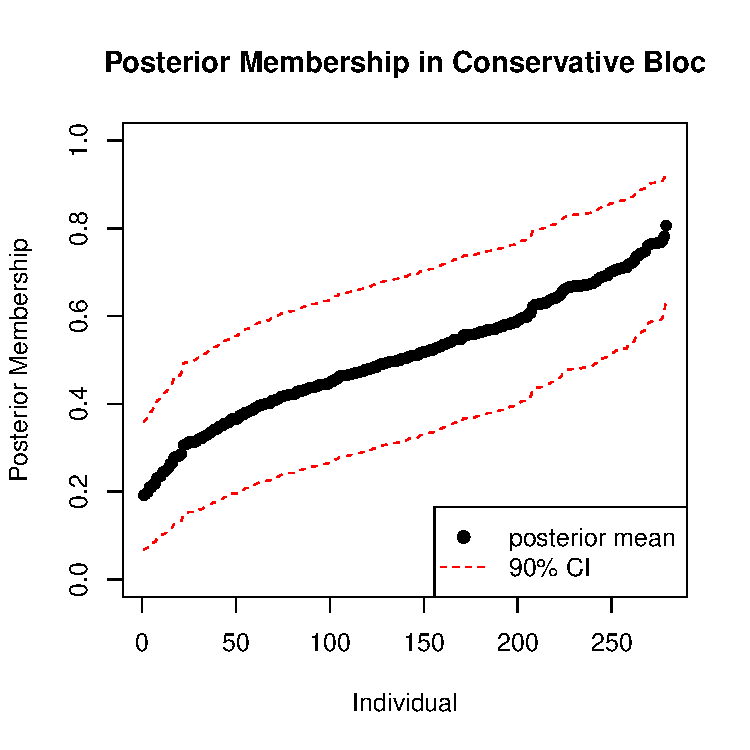
\includegraphics[width=\maxwidth]{figure/posteriorMem-1} 

}

\caption[We observe a relatively high rate of intra-individual mixing]{We observe a relatively high rate of intra-individual mixing\label{fig:posteriorMem}}
\end{figure}


\end{knitrout}


\subsection{Comparison of MCMC and Variational Results}
Comparing the results of the MCMC analysis by \cite{grossManriqueVallier} to the results from our variational analysis, we see they are very similar. In both analysis, we identify two dominant profiles- a conservative bloc and a liberal bloc- as well as a much smaller undecided faction. As can be seen in figure 2, the variational estimates of $\theta$ agree well with the MCMC esetimates.

Since Gross and Manrique-Vallier utilize a fully Bayesian specification, they  are able to utilize a hypothesis testing framework with $\theta$ to find the most polarizing issues. Because the variational analysis only provides point estimates of $\theta$, we used Hellinger distances instead. However, both analyses agree that the three most polarizing statements are  \texttt{IND5}, \texttt{IND3} and \texttt{EQ7}.

Although the broad interpretation and estimates of $\theta$ agree, we do see differences in the estimates of $\alpha$. Gross and Manrique-Vallier report a posterior mean of $\alpha = \left(0.462, 0.285, 0.01 8\right)$ yielding relative frequencies of $\left(60.4\%, 37.3\%, 2.3\%\right)$ for the conservative, liberal and undecided bloc respectively. Although the ordering of the relative frequency matches, this implies a much lower level of intra-individual mixing and as well as a higher relative frequency for the conservative bloc than the variational estimates of $\hat \alpha= \left(3.617, 3.448, 0.029 \right)$ and relative frequency estimates of $\left(0.510, 0.486, 0.004\right)$.

\section{Conclusion}
In this tutorial, we only briefly introduced the ideas of mixed membership models. For more interested readers, \cite{Airoldi2014Handbook} provide a much deeper exposition of mixed membership models as well as a variety of different applications. 

We also provide a step-by-step guide for using \texttt{mixedMem} as well as some sample visualizations/interpretations which may be helpful to the user. From the political survey example, we see that the use of variational inference largely agrees with the more complicated MCMC procedure, and still provides reasonable and interpretable results.

By providing an R package for fitting mixed membership models, we aim to aid researchers who are studying problems where a mixed membership analysis is compelling, but have been otherwise dissuaded by the computational difficulties. We hope that this package extends the use of mixed membership models to a variety of new disciplines and interesting scientific problems.

\bibliographystyle{plainnat}
\bibliography{pl}

\end{document}
